\begin{figure}[ht]
\centering
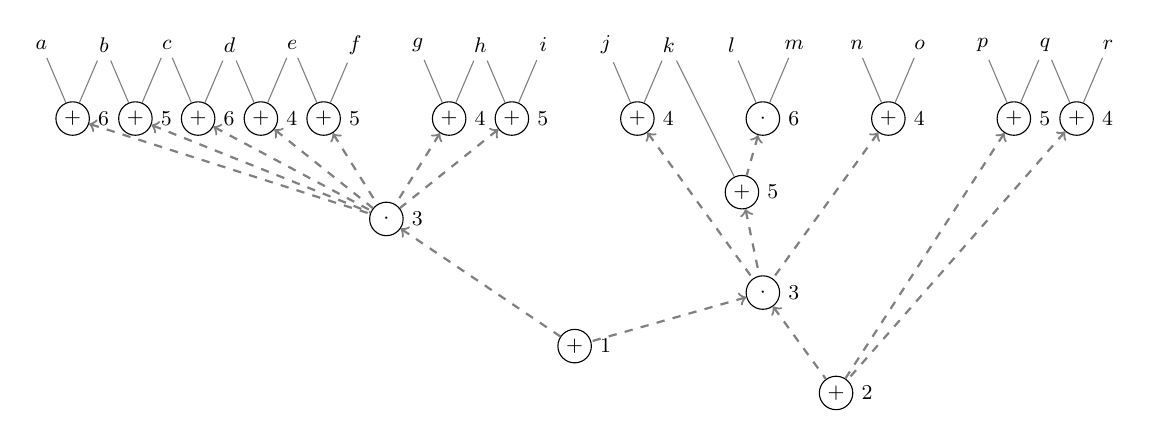
\begin{tikzpicture}[
	op/.style={circle, draw, inner sep=1.2pt, minimum size=5mm, font=\small},
	var/.style={font=\small},
	arg/.style={-, gray},
	prec/.style={<-, dashed, thick, gray},
	x=1.25cm, y=1cm,
	scale=0.85, every node/.style={transform shape}
]
% Operands (each symbol appears once, in one row)
\node[var] (a) at (0,0) {$a$};
\node[var] (b) at (0.75,0) {$b$};
\node[var] (c) at (1.5,0) {$c$};
\node[var] (d) at (2.25,0) {$d$};
\node[var] (e) at (3.0,0) {$e$};
\node[var] (f) at (3.75,0) {$f$};
\node[var] (g) at (4.5,0) {$g$};
\node[var] (h) at (5.25,0) {$h$};
\node[var] (i) at (6.0,0) {$i$};
\node[var] (j) at (6.75,0) {$j$};
\node[var] (k) at (7.5,0) {$k$};
\node[var] (l) at (8.25,0) {$l$};
\node[var] (m) at (9.0,0) {$m$};
\node[var] (n) at (9.75,0) {$n$};
\node[var] (o) at (10.5,0) {$o$};
\node[var] (p) at (11.25,0) {$p$};
\node[var] (q) at (12.0,0) {$q$};
\node[var] (r) at (12.75,0) {$r$};

% (a+b+c+d+e+f)
\node[op, label=right:{\small 6}] (p0) at (0.375,-1.1) {$+$};
\node[op, label=right:{\small 5}] (p1) at (1.125,-1.1) {$+$};
\node[op, label=right:{\small 6}] (p2) at (1.875,-1.1) {$+$};
\node[op, label=right:{\small 4}] (p3) at (2.625,-1.1) {$+$};
\node[op, label=right:{\small 5}] (p4_new) at (3.375,-1.1) {$+$};

% (g+h+i)
\node[op, label=right:{\small 4}] (p4) at (4.875,-1.1) {$+$};
\node[op, label=right:{\small 5}] (p5) at (5.625,-1.1) {$+$};

% (j+k+(l+m)) with inner (l+m)
\node[op, label=right:{\small 6}] (p6) at (8.625,-1.1) {$\cdot$};
\node[op, label=right:{\small 5}] (p7) at (8.375,-2.2) {$+$};
\node[op, label=right:{\small 4}] (p8) at (7.125,-1.1) {$+$};

% (n+o)
\node[op, label=right:{\small 4}] (p9) at (10.125,-1.1) {$+$};

% (p+q+r)
\node[op, label=right:{\small 5}] (p10) at (11.625,-1.1) {$+$};
\node[op, label=right:{\small 4}] (p11) at (12.375,-1.1) {$+$};

% Multiplications
\node[op, label=right:{\small 3}] (t1) at (4.125,-2.6) {$\cdot$};
\node[op, label=right:{\small 3}] (t2) at (8.625,-3.7) {$\cdot$};

% Top-level additions
\node[op, label=right:{\small 1}] (pt1) at (6.375,-4.5) {$+$};
\node[op, label=right:{\small 2}] (pt2) at (9.5,-5.2) {$+$};

% Argument edges (not precedence constraints)
\draw[arg] (a) -- (p0);
\draw[arg] (b) -- (p0);
\draw[arg] (b) -- (p1);
\draw[arg] (c) -- (p1);
\draw[arg] (c) -- (p2);
\draw[arg] (d) -- (p2);
\draw[arg] (d) -- (p3);
\draw[arg] (e) -- (p3);
\draw[arg] (e) -- (p4_new);
\draw[arg] (f) -- (p4_new);

\draw[arg] (g) -- (p4);
\draw[arg] (h) -- (p4);
\draw[arg] (h) -- (p5);
\draw[arg] (i) -- (p5);

\draw[arg] (l) -- (p6);
\draw[arg] (m) -- (p6);
\draw[arg] (k) -- (p7);
\draw[arg] (j) -- (p8);
\draw[arg] (k) -- (p8);

\draw[arg] (n) -- (p9);
\draw[arg] (o) -- (p9);

\draw[arg] (p) -- (p10);
\draw[arg] (q) -- (p10);
\draw[arg] (q) -- (p11);
\draw[arg] (r) -- (p11);

% Precedence arrows (only when forced, reversed direction)
\draw[prec] (p0) -- (t1);
\draw[prec] (p1) -- (t1);
\draw[prec] (p2) -- (t1);
\draw[prec] (p3) -- (t1);
\draw[prec] (p4_new) -- (t1);
\draw[prec] (p4) -- (t1);
\draw[prec] (p5) -- (t1);

\draw[prec] (p6) -- (p7);
\draw[prec] (p7) -- (t2);
\draw[prec] (p8) -- (t2);
\draw[prec] (p9) -- (t2);

\draw[prec] (t1) -- (pt1);
\draw[prec] (t2) -- (pt1);

\draw[prec] (t2) -- (pt2);
\draw[prec] (p10) -- (pt2);
\draw[prec] (p11) -- (pt2);
\end{tikzpicture}
\caption{Expression tree for $E = (a+b+c+d+e+f)\cdot(g+h+i) + (j+k+l\cdot m)\cdot(n+o) + (p+q+r)$. Each arrow denotes a precedence constraint. The numbers next to the operators denote an example valid ranking of the edges of the path graph, which corresponds to a valid parallel evaluation schedule for the expression. When executing the expression in parallel, at each time step, the colors are processed in an descending order.}
\label{fig:expression-tree-example}
\end{figure}
